\documentclass[]{beamer}

\usepackage{polyglossia}
\setdefaultlanguage{french}

\setmainfont{Tribun ADF Std}
\setsansfont{Tribun ADF Std}
\setmonofont{Fira Code}

\usepackage{soul}
\usepackage{microtype}
\usepackage{csquotes}
\usepackage{default}
\usepackage{hyperref}
\hypersetup{colorlinks=true}
\usetheme{simple}
\usepackage{graphicx}
\usepackage[justification=centering]{caption}
\usepackage{subcaption}
\usepackage{listings}
\usepackage{pstricks}
\usepackage{booktabs}
\captionsetup[subfigure]{labelformat=empty}
\captionsetup[figure]{labelformat=empty}
\setbeamertemplate{caption}{\raggedright\insertcaption\par}
\setbeamerfont{frametitle}{size=\LARGE}
\newfontfamily\DejaSans{DejaVu Sans}
\setbeamerfont{title}{family=\texttt,size=\huge}
%\usepackage[scale=2]{ccicons}
%\newfontfamily\unicodefun[Ligatures=TeX]{Symbola}
%\newfontfamily\unicodefun{Droid Sans}


\lstdefinelanguage{JavaScript}{
    keywords={typeof, new, true, false, catch, function, return, null, catch, switch, var, if, in, while, do, else, case, break},
    keywordstyle=\color{blue}\bfseries,
    ndkeywords={class, export, boolean, throw, implements, import, this},
    ndkeywordstyle=\color{darkgray}\bfseries,
    identifierstyle=\color{black},
    sensitive=false,
    comment=[l]{//},
    morecomment=[s]{/*}{*/},
    commentstyle=\color{purple}\ttfamily,
    stringstyle=\color{red}\ttfamily,
    morestring=[b]',
    morestring=[b]"
}

\lstset{
    language=JavaScript,
    extendedchars=true,
    basicstyle=\footnotesize\ttfamily,
    showstringspaces=false,
    showspaces=false,
    numberstyle=\footnotesize,
    numbersep=9pt,
    tabsize=2,
    breaklines=true,
    showtabs=false,
    captionpos=b
}

\title{Exécution répartie de partitions interactives}
\subtitle{}
\date{}
\author{Jean-Michaël Celerier$\mathsf{^{1,2}}$~\\ Myriam Desainte-Catherine$\mathsf{^{2}}$~\\ Jean-Michel Couturier$\mathsf{^{1}}$}
\institute{1. Blue Yeti --- 2. SCRIME / LaBRI}
\titlegraphic{
    
\includegraphics[width=0.2\textwidth]{images/logobl.png} \vspace{1cm}
    
\includegraphics[width=0.5\textwidth]{images/scrime.jpg}}
\usepackage{tikz}

\newsavebox{\codebox}% For storing listings
\begin{document}
\maketitle
\begin{frame}
    \tableofcontents
\end{frame}

\section{Introduction}
\begin{frame}
    \frametitle{Problématique}
    \Large
    \begin{itemize}
        \item Jouer A  sur les machines 1 et 2, B sur la machine 3.
        \item 
    \end{itemize}
\end{frame}

\begin{frame}
    \Large
    \begin{figure}
    	\centering
    	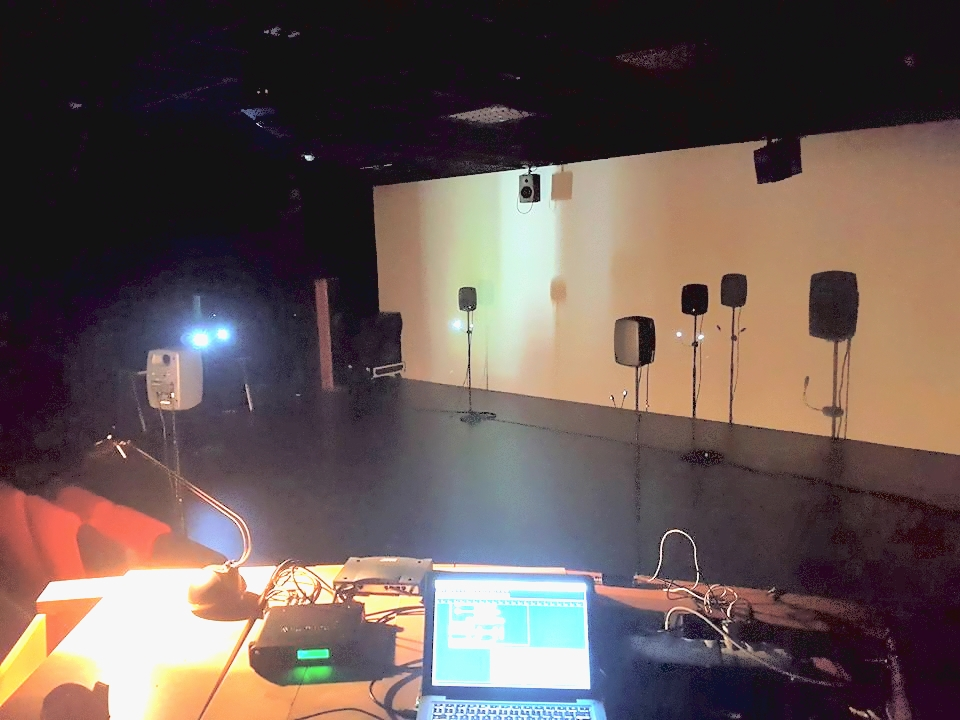
\includegraphics[width=0.9\textwidth]{images/quarre.jpg}
    	\caption{Quarrè (© Pierre Cochard)}
    \end{figure}
\end{frame}

\begin{frame}
\Large
\begin{figure}
	\centering
	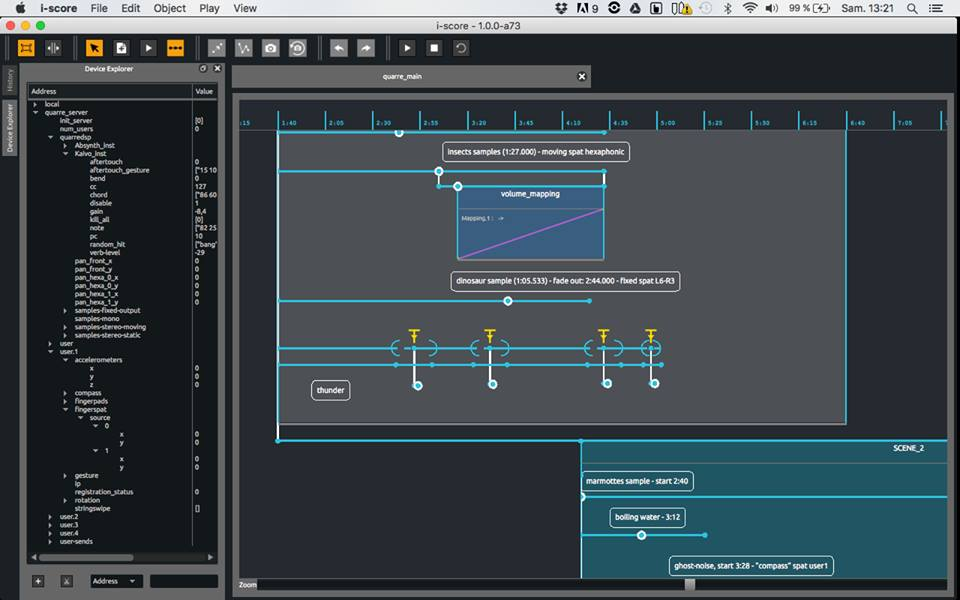
\includegraphics[width=0.9\textwidth]{images/quarre-2.jpg}
	\caption{Quarrè (© Pierre Cochard)}
\end{figure}
\end{frame}

\begin{frame}
\Large
\begin{figure}
	\centering
	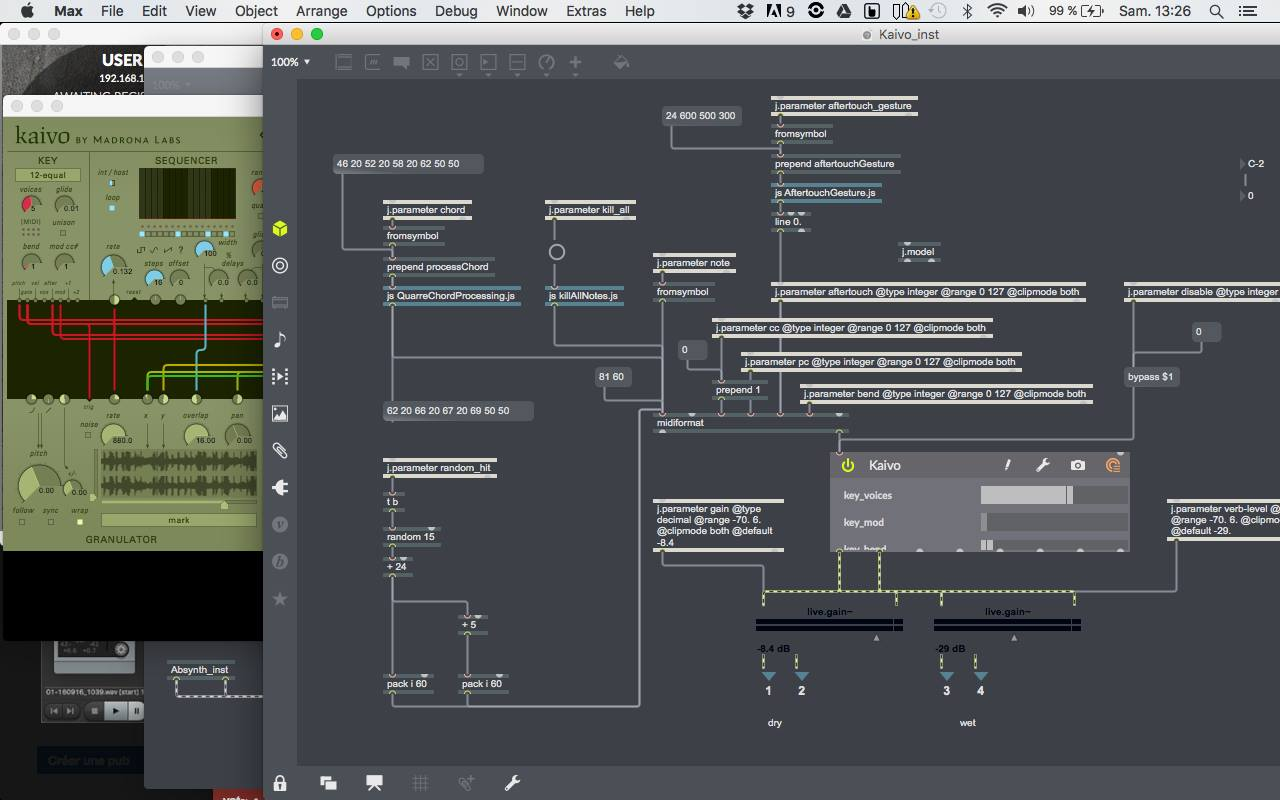
\includegraphics[width=0.9\textwidth]{images/quarre-3.jpg}
	\caption{Quarrè (© Pierre Cochard)}
\end{figure}
\end{frame}


\begin{frame}
    \frametitle{Existant}
    \Large
    \begin{itemize}
        \item Synchronisation d'horloge: NTP, PTP\dots
        \item Serveurs de son: NetJack
        \item Écriture et jeu répartis: OhmStudio, Kiwi
    \end{itemize}
\end{frame}

\begin{frame}
\frametitle{Rappel d'i-score}
\begin{figure}
    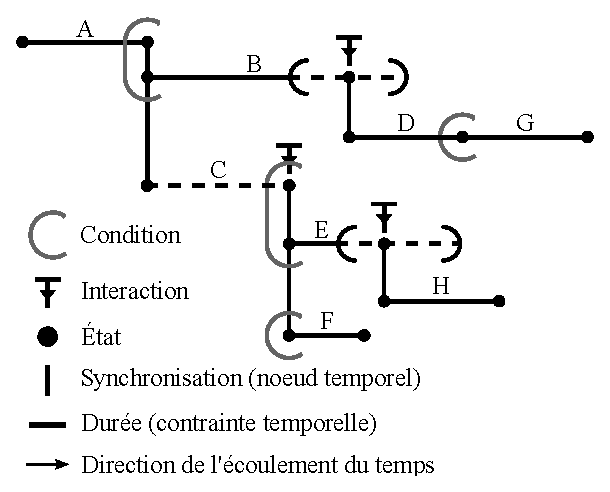
\includegraphics[width=0.8\textwidth]{scenarios/iscore-example.eps}
\end{figure}
\end{frame}

\section{Répartition}
\begin{frame}
\frametitle{Approche}
\begin{itemize}
    \item Séparation de l'écoulement du temps et de l'exécution des contenus.
\end{itemize}
\end{frame}

\subsection{Groupes}
\begin{frame}
\frametitle{Groupes}
{\Large Assurer l'indépendance vis-à-vis du matériel lors de l'écriture d'une partition.}
\begin{figure}
	\centering
	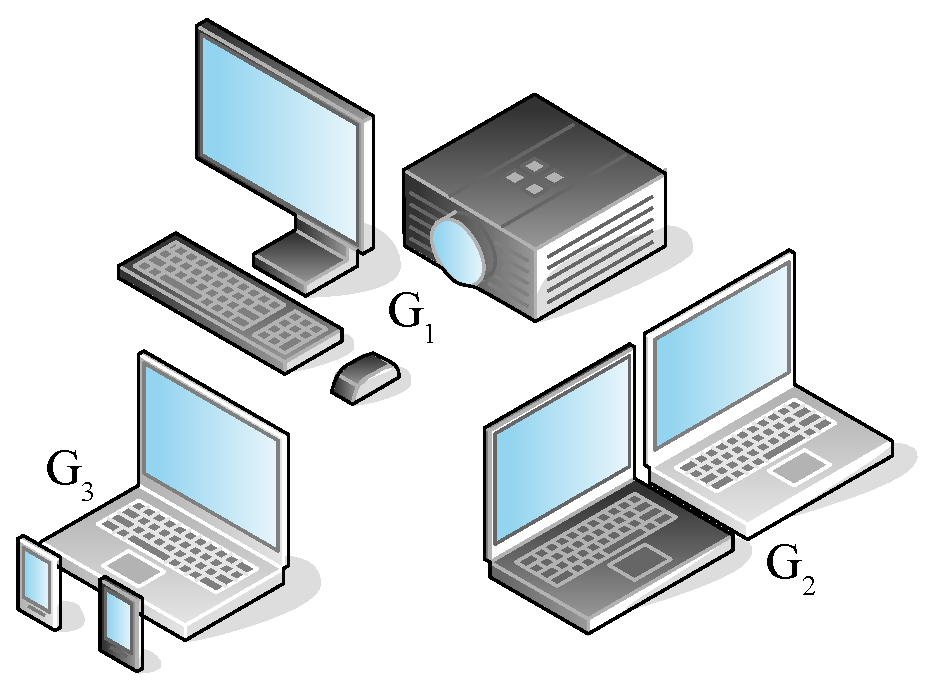
\includegraphics[width=0.6\textwidth]{images/groupes.eps}
	\caption{Groupes}
\end{figure}
\end{frame}


\subsection{Répartition des contenus}
\begin{frame}
\frametitle{Répartition des contenus}
{\Large Pour un agencement de structures temporelles donné, quelles sont les exécutions pouvant être définies ?}

\begin{itemize}
    \item<1> \textbf{Libre} : chaque machine exécute indépendamment.
    \item<1> \textbf{Partagée} : les temporalités sont identiques, les contenus changent.
    \item<1> \textbf{Mixte} : Les temporalités sont identiques au sein d'un groupe.
\end{itemize}
\end{frame}

\section{Synchronisation des interactions}
\begin{frame}
\frametitle{Interactions possibles}
\Large
\begin{itemize}
	\item<1> Points d'interaction
	\item<2> Conditions
	\item<3> Contrôle de la vitesse d'exécution 
\end{itemize}
\end{frame}


\begin{frame}
\frametitle{Exécution libre}
\begin{figure}
    \centering
    \begin{tikzpicture}
    \fill (0, 0.141497) circle (0.075) ; % State.0 
\fill (0, 0.141393) circle (0.075) ; % State.1 
\fill (3.02682, 0.141393) circle (0.075) ; % State.2 
\fill (5, 0.141393) circle (0.075) ; % State.4 
\draw[line width=1pt] (0, 0.141497)  -- (0, 0.141393) ; % TimeNode.0 
\draw[line width=1pt] (3.02682, 0.141393)  -- (3.02682, 0.141393) ; % whim75dash50 
\draw[line width=1pt] (5, 0.141393)  -- (5, 0.141393) ; % them13ergo22 
\draw[line width=1pt] (0, 0.141393)  -- (1.69361, 0.141393) ; % wavy46flak3 
\draw[dashed,line width=1pt] (1.69361, 0.141393)  -- (3.02682, 0.141393) ; % wavy46flak3 
\draw[line width=0.7pt] (1.93361, 0.294393) arc(90:270:0.15) ; % wavy46flak3 
\draw[line width=1pt] (3.02682, 0.141393)  -- (5, 0.141393) ; % dock4chew40 

    \end{tikzpicture}
    \caption{Notation}
\end{figure}
\begin{figure}
    \centering
    \begin{tikzpicture}
    \fill (0, 0.0104813) circle (0.075) ; % State.0 
\fill (0, 0.0104807) circle (0.075) ; % State.1 
\fill (2.68116, 0.0104807) circle (0.075) ; % State.2 
\fill (5, 0.0104807) circle (0.075) ; % State.4 
\draw[line width=1pt] (0, 0.0104813)  -- (0, 0.0104807) ; % TimeNode.0 
\draw[line width=1pt] (2.68116, 0.0104807)  -- (2.68116, 0.0104807) ; % whim75dash50 
\draw[line width=1pt] (5, 0.0104807)  -- (5, 0.0104807) ; % them13ergo22 
\draw[line width=1pt] (0, 0.0104807)  -- (2.68116, 0.0104807) ; % wavy46flak3 
\draw[line width=1pt] (2.68116, 0.0104807)  -- (5, 0.0104807) ; % dock4chew40 

    \end{tikzpicture}
    \caption{Déroulement sur la machine 1}
\end{figure}
\begin{figure}
    \centering
    \begin{tikzpicture}
    \fill (0, 0.0104814) circle (0.075) ; % State.0 
\fill (0, 0.0104808) circle (0.075) ; % State.1 
\fill (3.38811, 0.0104808) circle (0.075) ; % State.2 
\fill (5, 0.0104808) circle (0.075) ; % State.4 
\draw[line width=1pt] (0, 0.0104814)  -- (0, 0.0104808) ; % TimeNode.0 
\draw[line width=1pt] (3.38811, 0.0104808)  -- (3.38811, 0.0104808) ; % whim75dash50 
\draw[line width=1pt] (5, 0.0104808)  -- (5, 0.0104808) ; % them13ergo22 
\draw[line width=1pt] (0, 0.0104808)  -- (3.38811, 0.0104808) ; % wavy46flak3 
\draw[line width=1pt] (3.38811, 0.0104808)  -- (5, 0.0104808) ; % dock4chew40 

    \end{tikzpicture}
    \caption{Déroulement sur la machine 2}
\end{figure}
\end{frame}
\begin{frame}
\frametitle{Exécution partagée}
\begin{figure}
    \centering
    \begin{tikzpicture}
    
\draw[line width=1pt] (0, 0.655491)  -- (0, 0.653257) ; % TimeNode.0 
\draw[line width=1pt] (1.26282, 0.655491)  -- (1.26282, 0.655491) ; % whim75dash50 
\draw[line width=1pt] (2.94308, 0.655491)  -- (2.94308, 0.655491) ; % them13ergo22 
\draw[line width=1pt,color=cyan] (0, 0.655491)  -- (0.138662, 0.655491) ; % wavy46flak3 
\draw[dashed,line width=1pt,color=cyan] (0.138662, 0.655491)  -- (1.26282, 0.655491) ; % wavy46flak3 
\draw[line width=0.7pt,color=cyan] (0.378662, 0.808491) arc(90:270:0.15) ; % wavy46flak3 
\draw[line width=1pt,color=cyan] (0, 0.555491)  -- (1.26282, 0.555491)  -- (1.26282, -0.444509)  -- (0, -0.444509)  -- (0, 0.555491) ;
\draw[line width=1pt,color=cyan] (0, -0.444509)  -- (1.26282, 0.555491) ;
\draw[line width=1pt,color=orange] (1.26282, 0.655491)  -- (2.94308, 0.655491) ; % dock4chew40 
\draw[line width=1pt,color=orange] (1.26282, 0.555491)  -- (2.94308, 0.555491)  -- (2.94308, -0.444509)  -- (1.26282, -0.444509)  -- (1.26282, 0.555491) ;
\draw[line width=1pt,color=orange] (1.26282, -0.444509)  -- (2.94308, 0.555491) ;

\fill (0, 0.65508) circle (0.075) ; % State.0 
\fill (0, 0.655491) circle (0.075) ; % State.1 
\fill (1.26282, 0.655491) circle (0.075) ; % State.2 
\fill (2.94308, 0.655491) circle (0.075) ; % State.4 
\fill (0, 0.653257) circle (0.075) ; % State.5 
    \end{tikzpicture}
    \caption{Notation}
\end{figure}
\begin{figure}
    \centering
    \begin{tikzpicture}
    
\draw[line width=1pt] (0, 0.0104813)  -- (0, 0.0104807) ; % TimeNode.0 
\draw[line width=1pt] (3.30592, 0.0104807)  -- (3.30592, 0.0104807) ; % whim75dash50 
\draw[line width=1pt] (5, 0.0104807)  -- (5, 0.0104807) ; % them13ergo22 
\draw[line width=1pt] (0, 0.0104807)  -- (3.30592, 0.0104807) ; % wavy46flak3 
\draw[line width=1pt,color=orange] (3.30592, 0.0104807)  -- (5, 0.0104807) ; % dock4chew40 
\draw[line width=1pt,color=orange] (3.30592, -0.0895193)  -- (5, -0.0895193)  -- (5, -1.08952)  -- (3.30592, -1.08952)  -- (3.30592, -0.0895193) ;
\draw[line width=1pt,color=orange] (3.30592, -1.08952)  -- (5, -0.0895193) ;

\fill (0, 0.0104813) circle (0.075) ; % State.0 
\fill (0, 0.0104807) circle (0.075) ; % State.1 
\fill (3.30592, 0.0104807) circle (0.075) ; % State.2 
\fill (5, 0.0104807) circle (0.075) ; % State.4 
    \end{tikzpicture}
    \caption{Déroulement sur la machine 1}
\end{figure}
\begin{figure}
    \centering
    \begin{tikzpicture}
    \fill (0, 0.0104813) circle (0.075) ; % State.0 
\fill (0, 0.0104807) circle (0.075) ; % State.1 
\fill (3.30592, 0.0104807) circle (0.075) ; % State.2 
\fill (5, 0.0104807) circle (0.075) ; % State.4 
\draw[line width=1pt] (0, 0.0104813)  -- (0, 0.0104807) ; % TimeNode.0 
\draw[line width=1pt] (3.30592, 0.0104807)  -- (3.30592, 0.0104807) ; % whim75dash50 
\draw[line width=1pt] (5, 0.0104807)  -- (5, 0.0104807) ; % them13ergo22 
\draw[line width=1pt] (0, 0.0104807)  -- (3.30592, 0.0104807) ; % wavy46flak3 
\draw[line width=1pt] (0, -0.0895193)  -- (3.30592, -0.0895193)  -- (3.30592, -1.08952)  -- (0, -1.08952)  -- (0, -0.0895193) ;
\draw[line width=1pt] (0, -1.08952)  -- (3.30592, -0.0895193) ;
\draw[line width=1pt] (3.30592, 0.0104807)  -- (5, 0.0104807) ; % dock4chew40 

    \end{tikzpicture}
    \caption{Déroulement sur la machine 2}
\end{figure}
\end{frame}
\begin{frame}
\frametitle{Exécution mixte}
\end{frame}

\subsection{Synchronisation}
\begin{frame}
\frametitle{Synchronisation}
\Large
Plusieurs aspects : 
\large
\begin{itemize}
	\item \textbf{Latence} : délai des interactions.
	\item \textbf{Simultanéité} : la fin de $A$ concorde avec le début de $B$.
	\item Respect de l'\textbf{ordre des opérations} de la partition.
\end{itemize}
~\\
\Large Quatres modes pour les points d'interaction : 
\large
\begin{table}
	\begin{tabular}{c|c}
	Synchrone compensé & Synchrone non-compensé \\
	\midrule
	Asynchrone compensé & Asynchrone non-compensé
	\end{tabular}
\end{table}

\end{frame}

\begin{frame}
\frametitle{Compensation de latence}
\begin{figure}
	\centering
	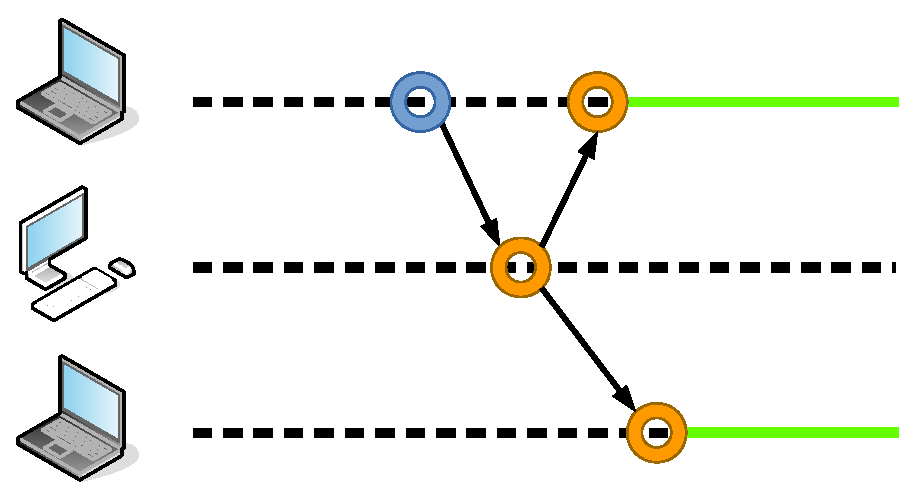
\includegraphics[width=\textwidth]{draw/noncompensated.eps}
	\caption{Pas de compensation de latence}
\end{figure}
\end{frame}

\begin{frame}
\frametitle{Compensation de latence}
\begin{figure}
	\centering
	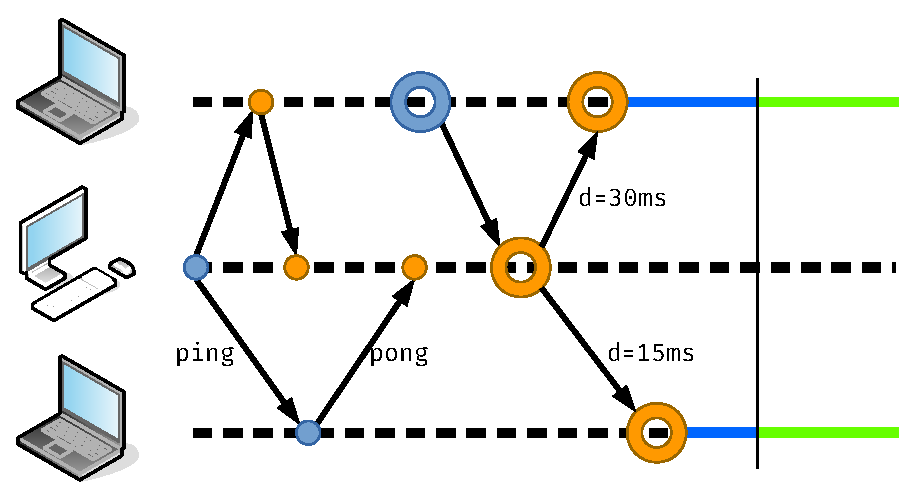
\includegraphics[width=\textwidth]{draw/compensated.eps}
	\caption{Compensation de latence}
\end{figure}
\end{frame}

\begin{frame}
\frametitle{Ordonnancement}
\centering
\Large
\begin{figure}
\begin{tikzpicture}[scale=2]
\fill (0, 18.8497) circle (0.075) ; % State.0 
\fill (2.85714, 18.8497) circle (0.075) ; % State.1 
\fill (2.85714, 16.9458) circle (0.075) ; % State.2 
\fill (5, 16.9458) circle (0.075) ; % State.3 
\fill (0, 17.9625) circle (0.075) ; % State.4 
\fill (2.85714, 17.9625) circle (0.075) ; % State.5 
\draw[line width=1pt] (0, 18.8497)  -- (0, 17.9625) ; % TimeNode.0 
\draw[line width=1pt] (2.85714, 18.8497)  -- (2.85714, 16.9458) ; % rape75slim69 
\draw (2.85714, 19.0997) node {$T: G_2$}; % rape75slim69 
\draw[line width=1pt] (5, 16.9458)  -- (5, 16.9458) ; % yeah95slog61 
\draw[dashed,line width=1pt] (0, 18.8497)  -- (2.85714, 18.8497) ; % hues23yost3 
\draw (1.42857, 19.0497) node {$C_1: G_1$}; % hues23yost3 
\draw[line width=1pt] (2.85714, 16.9458)  -- (5, 16.9458) ; % owls78enos27 
\draw (3.92857, 17.1458) node {$C_3: G_3$}; % owls78enos27 
\draw[line width=1pt] (0, 17.9625)  -- (2.26143, 17.9625) ; % buoy59germ52 
\draw[dashed,line width=1pt] (2.2643, 17.9625)  -- (3.46, 17.9625) ; % buoy59germ52 
\draw[line width=0.7pt] (2.4, 18.1155) arc(90:270:0.15) ; % buoy59germ52 
\draw[line width=0.7pt] (3.3, 17.8125) arc(-90:90:0.15) ; % buoy59germ52 
\draw (1.42857, 18.1625) node {$C_4: G_4$}; % buoy59germ52 

\end{tikzpicture}
\caption{Un scénario réparti sur quatre groupes}
\end{figure}
\end{frame}

\begin{frame}
\frametitle{Ordonnancement}
\centering
\large
\begin{figure}
	\begin{tikzpicture}[scale=1.1]
	\fill (0, 33.0914) circle (0.075) ; % State.0 
\fill (2.11864, 33.0914) circle (0.075) ; % State.1 
\fill (2.11864, 32.2673) circle (0.075) ; % State.2 
\fill (4.33108, 32.2673) circle (0.075) ; % State.3 
\fill (0, 30.9876) circle (0.075) ; % State.6 
\fill (2.72881, 30.9876) circle (0.075) ; % State.7 
\fill (0, 28.1996) circle (0.075) ; % State.8 
\fill (2.74576, 28.1996) circle (0.075) ; % State.9 
\fill (2.74576, 27.2398) circle (0.075) ; % State.10 
\fill (5, 27.2398) circle (0.075) ; % State.11 
\fill (0, 29.5708) circle (0.075) ; % State.12 
\fill (2.67797, 29.5708) circle (0.075) ; % State.13 
\draw[line width=1pt] (0, 33.0914)  -- (0, 28.1996) ; % TimeNode.0 
\draw[line width=1pt] (2.11864, 33.0914)  -- (2.11864, 32.2673) ; % curs71died66 
\draw[line width=1pt] (4.33108, 32.2673)  -- (4.33108, 32.2673) ; % loge90nigh11 
\draw[line width=1pt] (2.72881, 30.9876)  -- (2.72881, 30.9876) ; % ruin7wine32 
\draw[line width=1pt] (2.74576, 28.1996)  -- (2.74576, 27.2398) ; % isle5oven35 
\draw[line width=1pt] (5, 27.2398)  -- (5, 27.2398) ; % well97hits87 
\draw[line width=1pt] (2.67797, 29.5708)  -- (2.67797, 29.5708) ; % ahem0slut83 
\draw[dashed,line width=1pt] (0, 33.0914)  -- (2.11864, 33.0914) ; % tori2goat96 
\draw[dashed,line width=1pt] (2.11864, 32.2673)  -- (4.33108, 32.2673) ; % fade89hike97 
\draw[dashed,line width=1pt] (0, 30.9876)  -- (2.72881, 30.9876) ; % yank31crux79 
\draw[dashed,line width=1pt] (0, 28.1996)  -- (2.74576, 28.1996) ; % babe53cots63 
\draw[line width=1pt] (2.74576, 27.2398)  -- (5, 27.2398) ; % word70many73 
\draw[line width=1pt] (0, 29.5708)  -- (2.01695, 29.5708) ; % oint38zinc35 
\draw[dashed,line width=1pt] (2.01695, 29.5708)  -- (3.21356, 29.5708) ; % oint38zinc35 
\draw[line width=0.7pt] (2.25695, 29.7238) arc(90:270:0.15) ; % oint38zinc35 
\draw[line width=0.7pt] (3.06356, 29.4208) arc(-90:90:0.15) ; % oint38zinc35 

\draw (2.11864, 33.3414) node {$T_e$}; % curs71died66 
\draw (4.33108, 32.5173) node {$T_2$}; % loge90nigh11 
\draw (2.72881, 31.2376) node (T1) {$T_1$}; % ruin7wine32 
\draw (2.74576, 28.4496) node (T3) {$T_3$}; % isle5oven35 
\draw (2.67797, 29.8208) node (T4) {$T_4$}; % ahem0slut83 
\draw (1.36441, 31.1876) node {$C_1: G_1$}; % yank31crux79 
\draw (3.87288, 27.4398) node {$C_3: G_3$}; % word70many73 

\draw (1.33898, 29.7708) node {$C_4: G_4$}; % oint38zinc35 

\draw (3.33108, 32.5173) node {$G_2$}; % loge90nigh11 
\draw (1.11864, 33.3414) node {$G_2$}; % curs71died66 
\draw (1.40, 28.4097) node {$G_3$}; % isle5oven35 
\draw (4.4, 31.95) node (M134) {$M_1, M_3, M_4$};

\draw [->] (M134) edge [bend left] (T1) ;
\draw [->] (M134) edge [bend left] (T3) ;
\draw [->] (M134) edge [bend left] (T4) ;

	\end{tikzpicture}
	\caption{Cas asynchrone: l'ordre n'est pas nécessairement respecté}
\end{figure}
\end{frame}

\begin{frame}
\frametitle{Ordonnancement}
\centering
\large
\begin{figure}
\begin{tikzpicture}[scale=1.1]
\fill (0, 33.0914) circle (0.075) ; % State.0 
\fill (2.11864, 33.0914) circle (0.075) ; % State.1 
\fill (2.11864, 32.2673) circle (0.075) ; % State.2 
\fill (4.33108, 32.2673) circle (0.075) ; % State.3 
\fill (0, 31.079) circle (0.075) ; % State.6 
\fill (2.72881, 31.079) circle (0.075) ; % State.7 
\fill (0, 28.0397) circle (0.075) ; % State.8 
\fill (2.74576, 28.0397) circle (0.075) ; % State.9 
\fill (2.74576, 27.2398) circle (0.075) ; % State.10 
\fill (5, 27.2398) circle (0.075) ; % State.11 
\fill (0, 29.5708) circle (0.075) ; % State.12 
\fill (2.67797, 29.5708) circle (0.075) ; % State.13 
\fill (2.72881, 30.6905) circle (0.075) ; % State.14 
\fill (2.67797, 29.1594) circle (0.075) ; % State.15 
\draw[line width=1pt] (0, 33.0914)  -- (0, 28.0397) ; % TimeNode.0 
\draw[line width=1pt] (2.11864, 33.0914)  -- (2.11864, 32.2673) ; % curs71died66 
\draw[line width=1pt] (4.33108, 32.2673)  -- (4.33108, 32.2673) ; % loge90nigh11 
\draw[line width=1pt] (2.72881, 31.079)  -- (2.72881, 30.6905) ; % ruin7wine32 
\draw[line width=1pt] (2.74576, 28.0397)  -- (2.74576, 27.2398) ; % isle5oven35 
\draw[line width=1pt] (5, 27.2398)  -- (5, 27.2398) ; % well97hits87 
\draw[line width=1pt] (2.67797, 29.5708)  -- (2.67797, 29.1594) ; % ahem0slut83 
\draw[dashed,line width=1pt] (0, 33.0914)  -- (2.11864, 33.0914) ; % tori2goat96 
\draw[dashed,line width=1pt] (2.11864, 32.2673)  -- (4.33108, 32.2673) ; % fade89hike97 
\draw[dashed,line width=1pt] (0, 31.079)  -- (2.72881, 31.079) ; % yank31crux79 
\draw[dashed,line width=1pt] (0, 28.0397)  -- (2.74576, 28.0397) ; % babe53cots63 
\draw[line width=1pt] (2.74576, 27.2398)  -- (5, 27.2398) ; % word70many73 
\draw[line width=1pt] (0, 29.5708)  -- (2.01695, 29.5708) ; % oint38zinc35 
\draw[dashed,line width=1pt] (2.01695, 29.5708)  -- (3.21356, 29.5708) ; % oint38zinc35 
\draw[line width=0.7pt] (2.25695, 29.7238) arc(90:270:0.15) ; % oint38zinc35 
\draw[line width=0.7pt] (3.06356, 29.4208) arc(-90:90:0.15) ; % oint38zinc35 
\draw (1.33898, 29.7708) node {$C_4: G_4$}; % oint38zinc35 
\draw (1.11864, 33.3414) node {$G_2$}; % curs71died66 
\draw (1.4076, 28.2897) node {$G_3$}; % isle5oven35 

\draw (2.11864, 33.3414) node {$T_e$}; % curs71died66 
\draw (3.33108, 32.5173) node {$G_2$}; % loge90nigh11 
\draw (4.33108, 32.5173) node {$T_2$}; % loge90nigh11 
\draw (2.72881, 31.329) node (T1) {$T_1$}; % ruin7wine32 
\draw (2.74576, 28.2897) node (T3) {$T_3$}; % isle5oven35 
\draw (2.67797, 29.8208) node (T4) {$T_4$}; % ahem0slut83 
\draw (1.36441, 31.279) node {$C_1: G_1$}; % yank31crux79 
\draw (3.87288, 27.4398) node {$C_3: G_3$}; % word70many73 

\draw (4.4, 32) node (M14) {$M_1, M_4$}; 
		
\draw (3.2, 30.6905) node (M3a) {$M_3$}; 
\draw (3.2, 29.1594) node (M3b) {$M_3$}; 

\draw [->] (M14) edge [bend left] (T1) ;
\draw [->] (M14) edge [bend left] (T4) ;

\draw [->] (M3a) edge [bend left=60] (T3) ;
\draw [->] (M3b) edge [bend left] (T3) ;

\end{tikzpicture}
\caption{Cas synchrone: l'ordre est respecté}
\end{figure}
\end{frame}

\section{Implémentation}
\begin{frame}
\frametitle{Implémentation: utilisation dans i-score}
\end{frame}
\section{Conclusion}
\begin{frame}
    \frametitle{Conclusion}  
    \Large
    \begin{itemize}
        \item<1> Mécanisme de répartition des partitions écrites avec i-score.
    \end{itemize}

    Objectifs:
    \begin{itemize}
        \item<1> À court terme : permettre à une machine de rejoindre une exécution en cours de route.
        \item<2> À long terme : édition et exécution répartie en temps réel à plusieurs.
        \item<3> Intégration avec Ableton Link pour une précision plus élevée pour des scénarios audio.
    \end{itemize}
\end{frame}

\begin{frame}[allowframebreaks]%in case more than 1 slide needed
    
    %remove the icon
    \setbeamertemplate{bibliography item}{}
    
    %remove line breaks
    \setbeamertemplate{bibliography entry title}{}
    \setbeamertemplate{bibliography entry location}{}
    \setbeamertemplate{bibliography entry note}{}
    
    {\footnotesize
        \nocite{*}
        \bibliographystyle{IEEEtran}
        \bibliography{icmc2016}
    }
\end{frame}

\begin{frame}
    \frametitle{Liens} 
    \Large
    \begin{itemize}
        \setlength\itemsep{1em}
        \item \textbf{i-score} :~\\ {\small \url{www.i-score.org} }
        \item \textbf{Add-on réseau} :~\\ {\small \url{github.com/OSSIA/iscore-addon-network} }
    \end{itemize}
        
    \centering
    \vspace{2em}
    \Large{Merci ! Des questions ?}
    \vspace{2em}
    
    \small{Remerciements : Serge Chaumette, Pierre Cochard}
    
    \vspace{1em}
    
    \tiny{Utilise le thème Beamer 'simple' theme de Facundo Muñoz ainsi que les fontes Fira et ADF}
\end{frame}
\end{document}
